\documentclass[a4paper,12pt, titlepage]{article}
\usepackage{amssymb,amsthm,amsmath} %ams
\usepackage[finnish]{babel} %suomenkielinen tavutus
\usepackage[fixlanguage]{babelbib}
\selectbiblanguage{finnish}


\usepackage[T1]{fontenc} %skanditavutus
\usepackage[utf8x]{inputenc}        	% skandit utf-8 koodauksella
%\usepackage[ansinew]{inputenc}        	% skandit utf-8 koodauksella, kokeile tata, jos utf-8 ylla ei toimi.
\usepackage{graphicx}
%\usepackage{qtree}%yksinkertaiset puut
\usepackage{tikz}%vähän tehokkaampi grafiikkapaketti
\usepackage{cite}
\usepackage{url}
\usepackage[linesnumbered, boxed]{algorithm2e}
\let\oldnl\nl %vanha komento \nl talteen \oldnl
\newcommand{\nonl}{\renewcommand{\nl}{\let\nl\oldnl}} %poista rivinumero yhdeltä riviltä
%suomennoksia yo. paketille:
\renewcommand*{\algorithmcfname}{Algoritmi}
\renewcommand*{\listalgorithmcfname}{Lista algoritmeista}


\linespread{1.24} %1.24 olisi rivivali 1.5
\sloppy % Vahentaa tavutuksen tarvetta, "leventamalla" rivin keskella olevia valilyönteja.

% Lauseille, maaritelmille ja muille vastaaville voidaan maaritella omat ymparistöt
% jolloin niille saadaan yhtenainen ulkoasu
%\theoremstyle{definition}
\newtheoremstyle{break}
    {\topsep}{\topsep}%
    {\itshape}{}%
    {\bfseries}{}%
    {\newline}{}%
\theoremstyle{break}
\newtheorem{maar}{Maaritelma}[section] %Numeroidaan maaritelmat yms lukukohtaisesti. Juoksevan numeroinnin saa jattamalla [section]-option pois
\newtheorem{lause}[maar]{Lause}
\newtheorem{esimerkki}[maar]{Esimerkki}

% Yleisimmin kayttettaville komennoille voi maaritella lyhynnemerkintöja
% esimerkiksi
\newcommand{\R}{\mathbb{R}}
\newcommand{\abs}[1]{\vert #1 \vert} % Itseisarvo
\newcommand{\tab}[1][0.5cm]{\hspace*{#1}} % Sisennys
\newcommand{\code}[1]{\texttt{#1}} % Monospace-fontti koodille

\setlength\parindent{0pt} %uuden kappaleen sisennys

\title{Avaruusjakoon perustuvat tietorakenteet tietokonegrafiikassa}
\author{Timo Heinonen \\kandidaatintutkielma \\ tietojenkäsittelytiede \\ Turun yliopisto}
\date{Lokakuu 2016}
%\pagestyle{headings} 

\begin{document}

\thispagestyle{empty}
\begin{figure}

\includegraphics[width=3cm]{img/soihtu.png}
\vspace{4.0cm}
\end{figure}


\begin{center}\Large
Avaruusjakoon perustuvat tietorakenteet tietokonegrafiikassa
\end{center}

\begin{center}
Timo Heinonen\\
kandidaatintutkielma\\
marraskuu 2016
\end{center}

\begin{center}
Informaatioteknologian laitos\\
tietojenkäsittelytiede\\
Turun yliopisto\\
\end{center}

\begin{figure}[b]
\makebox[\textwidth]{
\includegraphics[width=\paperwidth]{img/footer.png}}
\vspace*{-5.0cm}
\end{figure}

\newpage
\pagenumbering{gobble}% Ei sivunumeroita
\thispagestyle{empty}
\section*{Tiivistelmä}
\newpage

\pagenumbering{arabic}% Sivunumerot takaisin

%\setcounter{tocdepth}{2} % Sisennys ToC:iin
\tableofcontents


\newpage
\section{Johdanto}

Kolmiulotteisen tietokonegrafiikkan tutkimuksella on ollut merkittävä vaikutus viihdeteollisuuteen, kuten animaatioelokuviin ja peleihin, sekä tietokoneavusteiseen suunnitteluun, esimerkiksi arkktehtuurin ja teollisuuden alalla.  Tietokonegrafiikka on osin jopa syrjäyttämässä perinteistä valokuvaustyötä: huonekalujätti Ikea on siirtynyt käyttämään myyntikuvastoissaan valtaosin tietokoneella generoituja kuvia valokuvien sijaan.\cite{ikea} Tietokonegrafiikan sovelluskohteet lisääntyvät jatkuvasti. Eräs aktiivinen tutkimuskohde on esimerkiksi tietokonegrafiikan tekniikoiden soveltaminen konenäköön \cite{hughes}\\

Grafiikan piirtämistä kolmiulotteisista malleista kaksiulotteisiksi kuviksi kutsutaan renderoinniksi. Renderoinnin lähtökohtana on kuvattava maisema (engl. \emph{scene}), joka sisältää objekteja ja valonlähteitä. Objektit ja valonlähteet on voitava mallintaa matemaattisesti, jotta niille voidaan määrittää sijainti ja suuntaus, ja jotta niiden välisiä etäisyyksiä ja suhteita voidaan laskea. Renderointi tapahtuu aina jostakin kuvakulmasta, ja tätä varten määritellään virtuaalinen kamera, jolla on oma sijaintinsa ja suuntauksensa maisemassa. Tämän jälkeen on selvitettävä, mitkä objektit kamera näkee, miten objekteihin osuvat valonsäteet vaikuttavat niiden väriin ja kuvan varjostukseen, ja lopuksi, mitkä värit projisoidaan kuvatason mihinkin pikseliin.\cite{janke}\\

1960-luvulla tietokonegrafiikkaa käytettiin lähinnä teollisuuden komponenttisuunnittelussa ja arkkitehtuurissa. Tietokoneella osattiin piirtää objektien ääriviivoja (engl. \emph{wireframe}), mutta varjostustekniikoita ei tunnettu. IBM:n tutkija Arthur Appel esitteli algoritmin, joka mallinsi valonsäteitä laskemalla suoran yhtälöitä kuvasta maisemaan ja siitä valonlähteisiin. Tämän tekniikan avulla voitiin piirtää yksinkertaisia varjostuksia.\cite{appel} Myöhemmin tästä Ray Tracing:iksi kutsutusta tekniikasta tuli erittäin suosittu.\\

Jo Appel totesi Ray Tracing -tekniikan olevan erittäin aikaavievä.\cite{appel} Vaikka tietokoneiden, ja varsinkin grafiikkaprosessoreiden laskentateho kasvaa jatkuvasti, ei grafiikan tuottaminen ole vieläkään halpaa tai nopeaa. Kuvista halutaan jatkuvasti realistisempia, ja yksityiskohtaisemmat kuvattavat mallit ja monimutkaiset valaisutekniikat vaativat erittäin paljon laskentatehoa. Esimerkiksi elokuvastudio Pixarin Monsterit-yliopisto -animaatioelokuvan piirtäminen vaati yli sata miljoonaa prosessorituntia.\cite{monsterit} Tämän takia tutkimuksen kohteena on ollut jo pitkään nopeampien renderointitekniikoiden kehittäminen.\\

1980-luvulla kehitettiin menetelmiä, joilla voitiin vähentää valonsäteiden ja maiseman osumatarkasteluiden määrää. Steven Rubin ja Turner Whitted esittelivät tekniikan, jossa maisema jaetaan esiprosessointivaiheessa hierarkisesti suuntaissärmiöihin ihmisen toimesta. Säteiden ja suuntaissärmiöiden osumia tarkastelemalla voitiin vähentää operaatioiden kokonaismäärää.\cite{rubin} Henry Fuchs et al. kehittivät toisen metodin, johon kuului myös esiprosessointivaihe, tällä kertaa tietokoneen suorittamana. Maiseman objektit oli jaettu pienempiin osiin, polygoneihin, joista valittiin binääripuun juureksi mahdollisimman keskellä maisemaa oleva. Tämän jälkeen binääripuuhun lisättiin polygoneja sillä perusteella, ovatko ne maisemassa vanhempansa etu- vai takapuolella. Näillä tekniikoilla renderointia saatiin nopeutettua siirtämällä työtä esiprosessointivaiheeseen.\cite{fuchs}  \\

Tässä tutkielmassa esitellään avaruuden jakamiseen perustuvia tietorakenteita, joilla kolmiulotteisten kuvien renderointia voidaan nopeuttaa. Luvussa 2 määritellään joitakin grafiikan peruskäsitteitä, sekä esitetään algoritmi Ray Tracing -tekniikalle. Luvussa 3 tutkitaan Binääristä avaruusjakoa, kd-puuta ja Bounding Volume -hierarkiaa, sekä niiden rakentamiseen ja läpikäyntiin liittyviä algoritmeja. Luvussa 4 selvitetään, miten kd-puuta voidaan käyttää Ray Tracing -algoritmin optimoimiseen.


\newpage
\section{Kolmiulotteisen tietokonegrafiikan peruskäsitteitä}
\subsection{Määritelmiä}

Kolmiulotteisten kuvien renderoinnin kohteena ovat \emph{objektit}, jotka mallintavat jotakin esinettä tai muotoa avaruudessa $\R^3$. Objektit voidaan esittää tietokoneen muistissa taulukkona pisteitä $P=(x,y,z)\;\epsilon\,\R^3$: esimerkiksi kolmiota voidaan kuvata kolmella pisteellä, ja palloa kahdella pisteellä, jotka esittävät sen keskipistettä ja yhtä pistettä sen pinnalla.\cite{angel}\\

Objektit jaetaan lähes kaikissa ei-triviaaleissa tapauksissa \emph{polygoneihin}. Polygoni, eli monikulmio $\gamma = \diamond P_1P_2...P_n, \; n > 2$, on samassa tasossa olevien kärkien $P_1,...,P_n$ muodostaman murtoviivan rajaama alue, jonka kärkien muodostamat janat $P_i P_{i+1}$ eivät leikkaa toisiaan.\cite{harju} Useimmiten grafiikkasovelluksissa ja -rajapinnoissa valitaan polygonien muodoksi kolmiot, sillä niiden kolme kärkeä muodostavat aina tason, ja grafiikkaprosessorit osaavat operoida kolmioilla erittäin nopeasti.\cite{angel}\\

Objektien sisäpuoli halutaan yleensä jättää huomioimatta, joten polygoneille on määriteltävä, kummalla puolella on niiden etupuoli. Kolmiot ovat tässäkin suhteessa hyvä valinta polygonien muodoksi, sillä kolmiolle $\triangle P_1P_2P_3$ voidaan helposti laskea etupuolen määrittävä normaali $n$ ristitulolla $(P_2-P_1) \times (P_3-P_2)$. Huomioitavaa on, että normaalin suunta riippuu siitä, missä järjestyksessä kärjet $P_1, P_2$ ja $P_3$ on määritelty.\cite{hughes}\\

Jotta voitaisiin tarkastella objektien, valonlähteiden, ja kuvakulman, eli \emph{kameran} välisiä suhteita ja suuntauksia avaruudessa, valitaan kolme koordinaatistoa, jotka on määritelty kolmella toisiinsa nähden kohtisuoralla kantavektorilla $(\vec{i},\vec{j},\vec{k})$. Jokaisella objektilla on \emph{lokaalikoordinaatisto}, joka sisältää objektin geometrian. Useimmiten origo sijoitetaan objektin keskipisteeseen. \emph{Maailmakoordinaatisto} kuvaa koko avaruutta, ja sisältää tietoa siitä, mihin objektien lokaalikoordinaatistojen origot on sijoitettu. Lopuksi tämä maisema kuvataan virtuaalisella kameralla, jolla on oma \emph{kamerakoordinaatistonsa}. Koordinaatistosta toiseen siirtyminen, koordinaatistojen skaalaus ja rotaatio voidaan toteuttaa lineaarikuvauksilla.\cite{janke}

\subsection{Ray Tracing -tekniikka}

Ray Tracing on renderointitekniikka, jolla voidaan piirtää erittäin fotorealistisia kuvia. Ray Tracing -tekniikka pyrkii mallintamaan valonsäteitä, jotka saavat alkunsa valonlähteistä, kulkevat avaruudessa ja osuvat objekteihin valaisten niitä, kimmoten niistä toisiin objekteihin ja muodostaen varjoja. Jotkut valonsäteet löytävät lopulta tiensä katsojan silmiin, eli kameraan. Koska olisi mahdotonta selvittää jokaisen valonsäteen kulkua avaruudessa, Ray Tracing -algoritmi ottaa huomioon vain ne säteet, jotka todella osuvat kameraan. Valonsäteitä seurataan siis käänteisessä järjestyksessä, kamerasta objekteihin, ja niistä valonlähteisiin.\cite{janke}\\

Ray Tracing -algoritmi muodostaa sille syötteenä annetusta kolmiulotteisesta maisemasta kameran sijainnin perusteella kaksiulotteisen kuvan. Jokaisen kuvatason pikselin läpi ammutaan säde $\vec{R}=O+t\vec{D}$, missä $t\,\epsilon\,\R$, $O$ on kameran sijainti maailmakoordinaatistossa ja normalisoitu vektori $\vec{D}$ kuvaa säteen kulkusuuntaa. Säteellä etsitään törmäyspistettä lähimmän objektin kanssa, eli sellaista mahdollisimman pientä arvoa $t$, että piste $P=O+t\vec{D}$ on jonkin objektin pinnalla. Tällöin osuman saaneen objektin piste $P$ voi näkyä kameraan, mikäli siihen osuu valoa. Osumakohdasta ammutaan uusi, varjostussäteeksi kutsuttu säde. Jos varjostussäde osuu suoraan tai kimmoten muista objekteista valonlähteeseen, lankeaa objektin pinnalle valoa.\cite{janke} Tekniikan pseudokoodi on esitetty algoritmissa \ref{algo_raytrace}.\\

\begin{algorithm}[htp]
\small
\KwIn{\\\texttt{kuvataso}: $x*y$ kokoinen taulukko pikseleitä \\
\texttt{maisema}: joukko valonlähteitä ja monikulmioihin jaettuja objekteja}
\KwOut{\\kolmiulotteinen maisema projisoituna \texttt{kuvataso}lle}
\BlankLine
\nonl \texttt{RAY\_TRACING(kuvataso, maisema)}:\\
\ForEach{pikseli $(x,y) \; \epsilon$ \textnormal{\texttt{kuvataso}}}{
  \texttt{etaisyys} $\gets \infty$ \\
  \ForEach{monikulmio $\epsilon$ \textnormal{\texttt{maisema}}}{
    Ammu säde $\vec{R}=O+t\vec{D}$ kamerasta pikselin läpi \textnormal{\texttt{maisema}}an \\
    \eIf{säde $\vec{R}$ osui monikulmioon pisteessä $P$ {\bf and} t < \textnormal{\texttt{etaisyys}}}{
	\texttt{etaisyys} $\gets t$\\ 
      	Valon määrä $V \gets 0$\\
	\ForEach{valonlähde $L$}{
	Ammu varjostussäde $\vec{R_s}=L-P$ valonlähdettä kohti\\
	Kasvata valosummaa $V$               
      }
      Aseta pikselin $(x,y)$ väri valosumman $V$ mukaisesti
    }{
      Aseta pikseli $(x,y)$ taustan väriseksi
    }
  }
}
\KwRet \texttt{kuvataso}
\caption{\texttt{RAY\_TRACING}}
\label{algo_raytrace}
\end{algorithm}


Algoritmin suoritusnopeutta rajoittaa se, että jokaista sädettä kohti on käytävä läpi kaikki maiseman polygonit ja testattava osuuko säde niihin. Säteiden ja polygonien leikkauksien määrittämiseen joudutaan joissain tapauksissa käyttämään jopa 95\% koko laskenta-ajasta.\cite{whitted} Algoritmia saataisiin siis nopeutettua huomattavasti, jos testattavien polygonien määrää jokaista sädettä kohti saataisiin vähennettyä. Yleisesti käytetty tapa leikkaustestien vähentämiseksi on muodostaa maisemasta hierarkinen tietorakenne ennen varsinaista renderointia. Tätä tietorakennetta läpikäymällä löydetään nopeasti polygoni, jonka pinnalla säteen ja objektin leikkauspiste $P$ on.\cite{rubin}


\newpage
\section{Avaruusjakopuut}
\subsection{Binäärinen avaruusjako}

Eräs suosittu avaruusjakoon perustuva tietorakenne on binäärinen avaruusjakopuu, eli \emph{BSP-puu} (engl. \emph{Binary Space Partitioning}). BSP-puu luodaan valitsemalla kolmiulotteisen maiseman  polygonijoukosta $\Gamma$ yksi polygoni $\gamma_k$, joka asetetaan puun juureksi. Polygonin $\gamma$ muodostama taso jakaa maiseman, ja siten polygonijoukon $\Gamma$, kahteen osaan $\Gamma_{k,+}$ ja $\Gamma_{k,-}$. Joukko $\Gamma_{k,+}$ sisältää polygonin $\gamma_k$ positiivisella puolella olevat polygonit, ja siten ne asetetaan BSP-puuhun juuren oikeaksi lapseksi. Vastaavasti joukko $\Gamma_{k,-}$ sisältää negatiivisella puolella olevat polygonit, ja kuuluvat polygonin $\gamma_k$ vasemmaksi lapseksi. Tämä jakavan polygonin valinta ja avaruuden jako suoritetaan rekursiivisesti BSP-puun lehdille, kunnes jokaisessa lehdessä on vain yksi polygoni.\cite{samet} BSP-puun rakentamisen pseudokoodi on esitelty algoritmissa \ref{algo_bsp}.\\

BSP-puuta ja sen solmuja voidaan esittää grafiikkasovelluksessa seuraavasti:\\\\%\cite{ranta}
\code{
class BSP\_Tree\\
\{\\
\tab BSP\_Node juuri\\
\}\\\\
class BSP\_Node\\
\{\\
\tab Polygon jakaja\\
\tab BSP\_Node* oikea\_lapsi\\
\tab BSP\_Node* vasen\_lapsi\\
\tab Polygon Polygonit[$\,$] \tab //joukko polygoneja, josta alipuut\\ 
\hspace*{5.65cm} muodostetaan\\
\}\\}

\begin{algorithm}[htp]
\small
\KwIn{\\
\texttt{BSP\_Node solmu}:\hspace{1.54cm} juurisolmu, josta puu rakennetaan\\
\texttt{Polygon monikulmiot[$\,$]}: monikulmiojoukko, josta alipuut rakennetaan}
\KwOut{\\BSP-puu, jonka juurena on solmu \texttt{node}}
\BlankLine
\nonl \texttt{RAKENNA\_BSP\_PUU(solmu, monikulmiot):\\}
 \texttt{jakaja} $\gets$ \texttt{VALITSE\_JAKAVA\_MONIKULMIO(monikulmiot)}\\
 \texttt{positiivinen\_joukko} $\gets \emptyset$\\
 \texttt{negatiivinen\_joukko} $\gets \emptyset$\\
 \ForEach{\textnormal{\texttt{$\gamma \, \epsilon$ monikulmiot}}}{
   \texttt{sijainti} $\gets$ \texttt{VERTAA($\gamma$, jakaja)}\\
  \uIf{\textnormal{\texttt{sijainti} = jakajan edessä}}{
   \texttt{positiivinen\_joukko} = \texttt{positiivinen\_joukko} $\cup\;\gamma$
  }
  \uElseIf{\textnormal{\texttt{sijainti} = jakajan takana}}{
   \texttt{negatiivinen\_joukko} = \texttt{negatiivinen\_joukko} $\cup\;\gamma$
  }
  \ElseIf{\textnormal{\texttt{sijainti} = leikkaa jakajan määrittämää tasoa}}{
   \texttt{JAA\_MONIKULMIO($\gamma$, jakaja, $\Gamma_{jakaja,+}$, $\Gamma_{jakaja,-}$)}\\
   \texttt{positiivinen\_joukko} = \texttt{positiivinen\_joukko} $\cup\;\Gamma_{jakaja,+}$\\
   \texttt{negatiivinen\_joukko} = \texttt{negatiivinen\_joukko} $\cup\;\Gamma_{jakaja,-}$
  }  
 }
\If{\textnormal{\texttt{positiivinen\_joukko}} $\neq \emptyset$}{
 \texttt{RAKENNA\_BSP\_PUU(solmu.oikea\_lapsi, positiivinen\_joukko)}
}
\If{\textnormal{\texttt{positiivinen\_joukko}} $\neq \emptyset$}{
 \texttt{RAKENNA\_BSP\_PUU(solmu.vasen\_lapsi, negatiivinen\_joukko)}
}

\caption{\texttt{RAKENNA\_BSP\_PUU \citep{ranta}}}\label{algo_bsp}
\end{algorithm}



\newpage
Kuvissa \ref{bsp1}-\ref{bsp3} on esitetty esimerkki BSP-puun muodostamisesta. Kuvassa \ref{bsp1} on yksinkertaisuuden vuoksi esitetty polygonit $A-F$ sisältävä maisema kaksiulotteisena. Kuvassa \ref{bsp2} ensimmäiseksi jakopolygoniksi on valittu $G$, jonka positiiviselle puolelle $\Gamma_{g,+}$ jäävät polygonit $A$, $B$ ja $C$, ja negatiiviselle puolelle $\Gamma_{g,-}$ polygonit $D$, $E$ ja $F$. Jaon g negatiivinen puoli saadaan jaettua loppuun asti ongelmitta valitsemalla jakopolygoniksi $E$, mutta jos positiivisella puolella valitaan jakopolygoniksi $B$, joudutaan polygoni $C$ jakamaan osiin $C_1$ ja $C_2$. Jakolinjan $b$ negatiiviselle puolelle jää vain yksi polygoni $C_2$, joten jaettavaksi jää vain $b$:n positiivinen puoli. Valitsemalla viimeiseksi jakopolygoniksi $A$ syntyy kuvan \ref{bsp3} mukainen BSP-puu.\\

\begin{figure}
 \centering
 \includegraphics[width=0.6\textwidth]{img/bsp1.png}
 \vspace{0.5cm}
 \caption{Joukko polygoneja tasossa}
 \label{bsp1}
\end{figure}

\begin{figure}
 \centering
 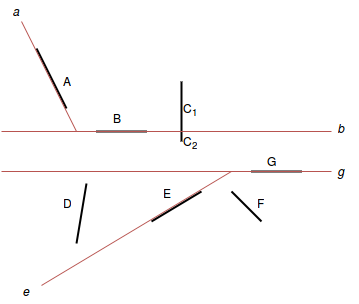
\includegraphics[width=0.6\textwidth]{img/bsp2.png}
 \vspace{0.5cm}
 \caption{Taso neljän jaon jälkeen}
 \label{bsp2}
\end{figure}

\begin{figure}
 \centering
 \begin{tikzpicture}[level/.style={sibling distance = 60mm/#1}]
  \node[circle,draw] (z){$G$}
    child {node [circle,draw] (a) {$E$}
     child {node [circle,draw] (b) {$D$}}
     child {node [circle,draw] (c) {$F$}}
    }
    child {node [circle,draw] (d) {$B$}
     child {node [circle,draw] (e) {$C_2$}}
     child {node [circle,draw] (f) {$A$}
      child[missing] {node {}}
      child {node [circle,draw] (g) {$C_1$}}}
    };
 \end{tikzpicture}
 \caption{Tasosta muodostettu BSP-puu}
 \label{bsp3}
\end{figure}

BSP-puun kokoon ja muotoon vaikuttaa suuresti avaruuden jakavan polygonin valinta. Pahimmassa tapauksessa kaikki polygonit $\Gamma\backslash\gamma_k$ jäävät polygonin $\gamma_k$ positiiviselle tai negatiiviselle puolelle jokaisella jaolla $k$. Tällöin puusta muodostuu pikemminkin ketjun muotoinen. Sama polygoni voi myös kuulua moneen BSP-puun alipuuhun, jos jonkun ylemmällä tasolla avaruuden jakavan polygonin $\gamma_k$ muodostama jakolinja leikkaa tätä polygonia.\cite{samet} Toinen lähestymistapa jakolinjalla oleviin polygoneihin on halkaista ne kahtia. Tämäkin tapa on epäedullinen, sillä se lisää maisemassa olevien polygonien määrää.\cite{ranta} Kun otetaan huomioon nämä rajoitteet, ei BSP-puun koolle voida antaa tarkkaa ylärajaa.\cite{hughes}\\

BSP-puuta rakennettaessa tavoitteena on muodostaa mahdollisimman tasapainoinen binääripuu valitsemalla jokaisella jakokerralla jakajaksi sellainen polygoni $\gamma_k$, jonka positiivisella ja negatiivisella puolella on likimain yhtä paljon polygoneja, eli $\abs{\Gamma_{k,+}} \approx \abs{\Gamma_{k,-}}$. Tällöin  $n$:n polygonin joukousta muodostetun BSP-puun syvyys olisi $O(\log n)$. Koska puun solmuja syntyy lisää, kun jakolinjan leikkaavat polygonit jaetaan kahtia, tai jakolinjalla oleva polygoni sisällytetään useaan alipuuhun, voidaan puun logaritmista tavoitesyvyyttä pitää vain alarajana.\cite{hughes} $n$ polygonia sisältävästä maisemasta rakennetun BSP-puun syvyys on siis $\Omega(\log n)$\\

BSP-puu voidaan rakentaa ennen renderointia esiprosessointivaiheessa. Renderointivaiheessa sitä voidaan käyttää vähentämään säde-polygoni leikkaustestien määrää. Kamerasta ammuttua sädettä verrataan ensin BSP-puun juurena toimivaan polygoniin. Jos säde leikkaa polygonin $\gamma_k$ muodostaman avaruuden jakavan tason, säde voi osua johonkin polygoniin molemmissa joukoissa ${\Gamma_{k,+}}$ ja ${\Gamma_{k,-}}$, eli joudutaan tarkastelemaan molempia alipuita. Jos säde ei leikkaa jakolinjaa, siirrytään tarkastelemaan vain toista alipuuta. Toistamalla säteiden ja avaruuden jakavien tasojen leikkauksia rekursiivisesti, päädytään lopulta BSP-puun juureen ja voidaan testata, osuuko säde polygoneihin.\cite{ranta}\\

\subsection{kd-puu}
\subsection{Bounding Volume -hierarkia}

\newpage
\section{Renderoinnin optimoiminen avaruusjakopuiden avulla}
\subsection{kd-puuta käyttävä Ray Tracing -algoritmi}
%Viittaus\cite{ranta},\cite{samet}
\cite{havran}

\newpage
\bibliographystyle{apalike-finnish} %bibplain vai apalike?
\bibliography{bibliography}
\listofalgorithms

\end{document}
